\documentclass[spanish,notitlepage,letterpaper, 12pt]{article} % para articulo en castellano
\usepackage[ansinew]{inputenc} % Acepta caracteres en castellano
\usepackage[spanish]{babel} % silabea palabras castellanas
\usepackage{url}
\usepackage{amsmath}
\usepackage{amsfonts}
\usepackage{float}
\usepackage{amssymb}
\usepackage[colorlinks=true,urlcolor=blue,linkcolor=blue]{hyperref} % navega por el doc
\usepackage{graphicx}
\usepackage{geometry}      % See geometry.pdf to learn the layout options.
\geometry{letterpaper}                   % ... or a4paper or a5paper or ...
%\geometry{landscape}                % Activate for for rotated page geometry
%\usepackage[parfill]{parskip}    % Activate to begin paragraphs with an empty line rather than an indent
\usepackage{epstopdf}
\usepackage{fancyhdr} % encabezados y pies de pg
\usepackage{pgf,pgfarrows,pgfnodes}
\usepackage{graphicx}

\renewcommand{\spanishtablename}{Cuadro}

\pagestyle{fancy}
\chead{\bfseries Tarea 3}
\lhead{} % si se omite coloca el nombre de la seccion
\rhead{ }
\lfoot{\it }
\cfoot{}
\rfoot{\thepage}

\voffset = -0.25in
\textheight = 9.0in
\textwidth = 6.5in
\oddsidemargin = 0.in
\headheight = 20pt
\headwidth = 6.5in
\renewcommand{\headrulewidth}{0.5pt}
\renewcommand{\footrulewidth}{0,5pt}
\DeclareGraphicsRule{.tif}{png}{.png}{`convert #1 `dirname #1`/`basename #1 .tif`.png}

\begin{document}
\title{Tarea 3 \\ Distribuciones Discretas}

\author{
\textbf{Erick Cervantes Mendieta} \\
\vspace{0.5cm}
\textnormal{Matr�cula: 2032430}\\
\textit{Modelos Probabilistas Aplicados}}
\date{Septiembre 2020}

\maketitle

%------------------------------------------------

\section{Presentaci�n de los datos}

Para esta tarea se analiz� el libro titulado ``The Singing Mouse Stories", el cual se encuentra disponible de manera gratuita en el sitio Web: \emph{Project Gutenberg} \cite{Mouse}. Se hizo un an�lisis en el programa R (Versi�n 4.0.2) \cite{LenguajeR} de la frecuencia en que aparece la letra \emph{e} en todo el libro, por ejemplo, en el t�tulo del libro podemos observar que dicha letra aparece en el lugar n�mero tres, luego se encuentran otras doce letras para aparecer de nuevo y finalmente se anotaron otras cinco letras para volver a tipear \emph{e}, un an�lisis parecido se hizo con la palabra \emph{singing}. Finalmente se presenta un an�lisis del n�mero de veces en que aparece la frase \emph{the singing mouse} en el texto.\\

\section{An�lisis de los datos}

La figura \ref{f1}(a) muestra el comportamiento de las veces en que fue apareciendo la letra e, en d�nde, a simple vista se podr�a decir que sigue una distribuci�n Geom�trica, sin embargo la primera barra podr�a causar un poco de confunsi�n, por lo que en la figura \ref{f1}(b), \ref{f1}(c) y \ref{f1}(d) se muestran algunas simulaciones de las distribuciones Geom�trica, Binomial y Binomial Negativa, respectivamente, utilizando algunos par�metros del libro utilizado. \\

Se puede concluir que al parecer la frecuencia con la que fue utilizada la letra \emph{e}, sigue una distribuci�n Geom�trica, aunque hace falta hacer un an�lisis m�s profundo para poder comprobar este supuesto.\\

\begin{figure}[]
\begin{center}
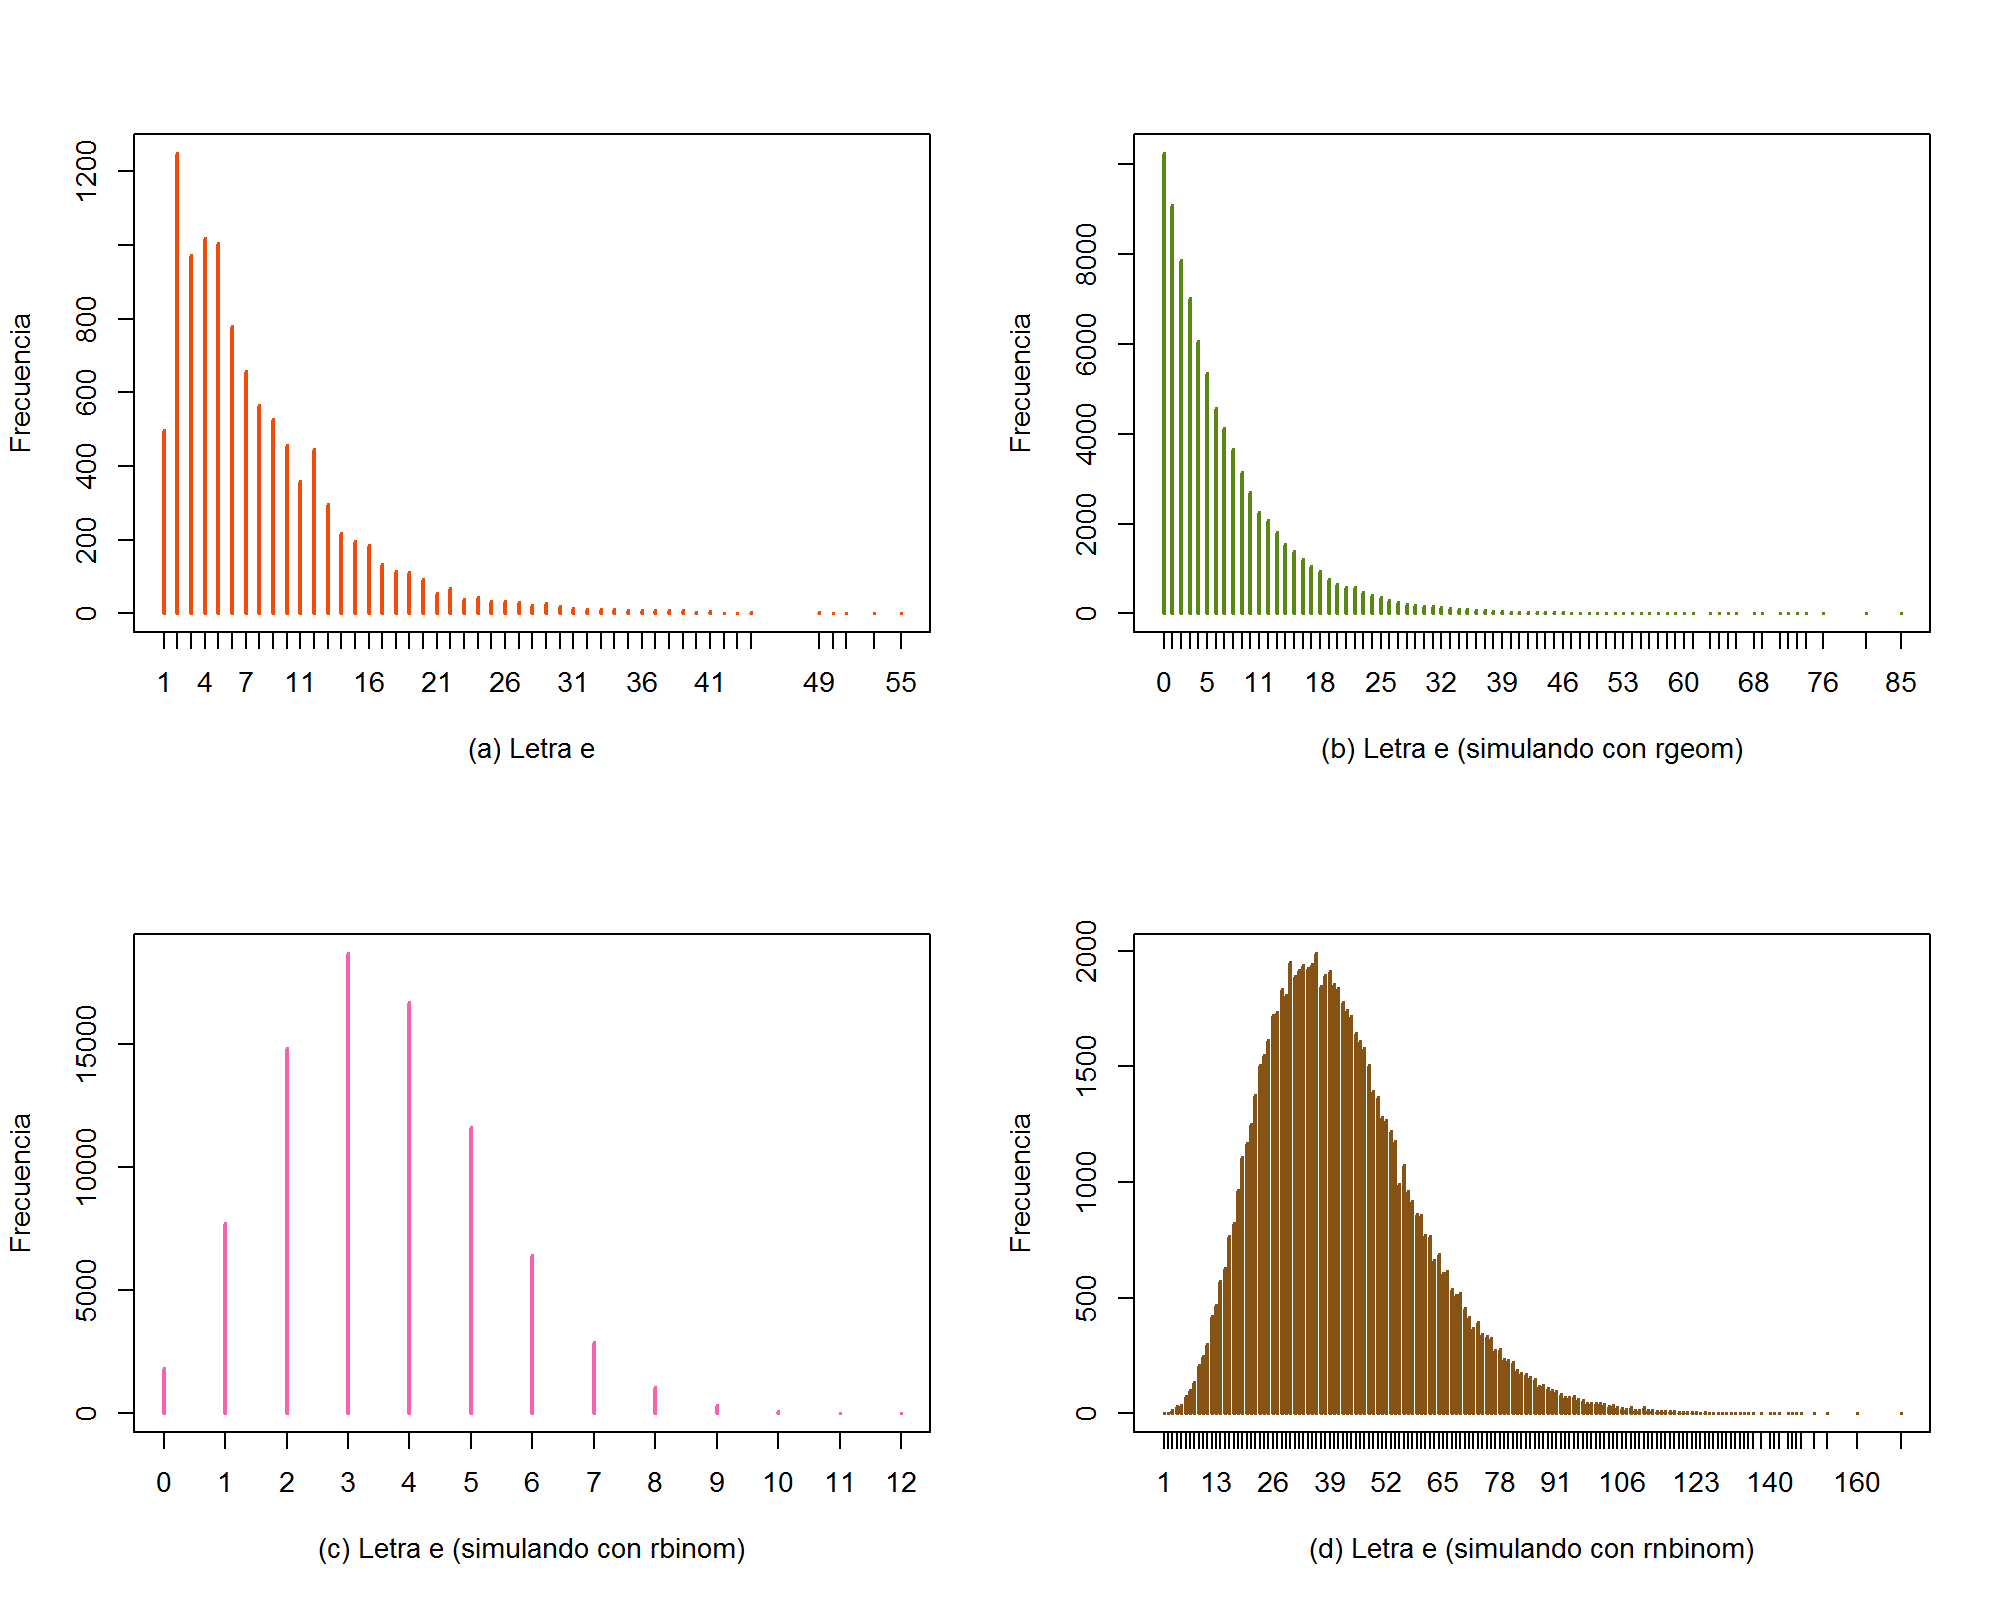
\includegraphics[width=15 cm]{FigModeloReporte/T3_e_todas.png}
\caption{Frecuencia de la letra \emph{e} utilizadas en el texto}\label{f1}
\end{center}
\end{figure}

En la figura \ref{f2}(a) se puede visualizar el n�mero de veces en la que fue apareciendo la palabra \emph{singing}, se puede observar que al parecer no sigue alguna distribuci�n de probabilidad discreta, ya que tiene un gran pico casi al inicio de la gr�fica, quiz� al suavizar un poco la gr�fica se podr�a observar algo m�s. Luego, se trato de simular como si fuera una Binomial, sin embargo no se pudo concluir visualmente que se siga dicha distribuci�n.\\

\begin{figure}[]
\begin{center}
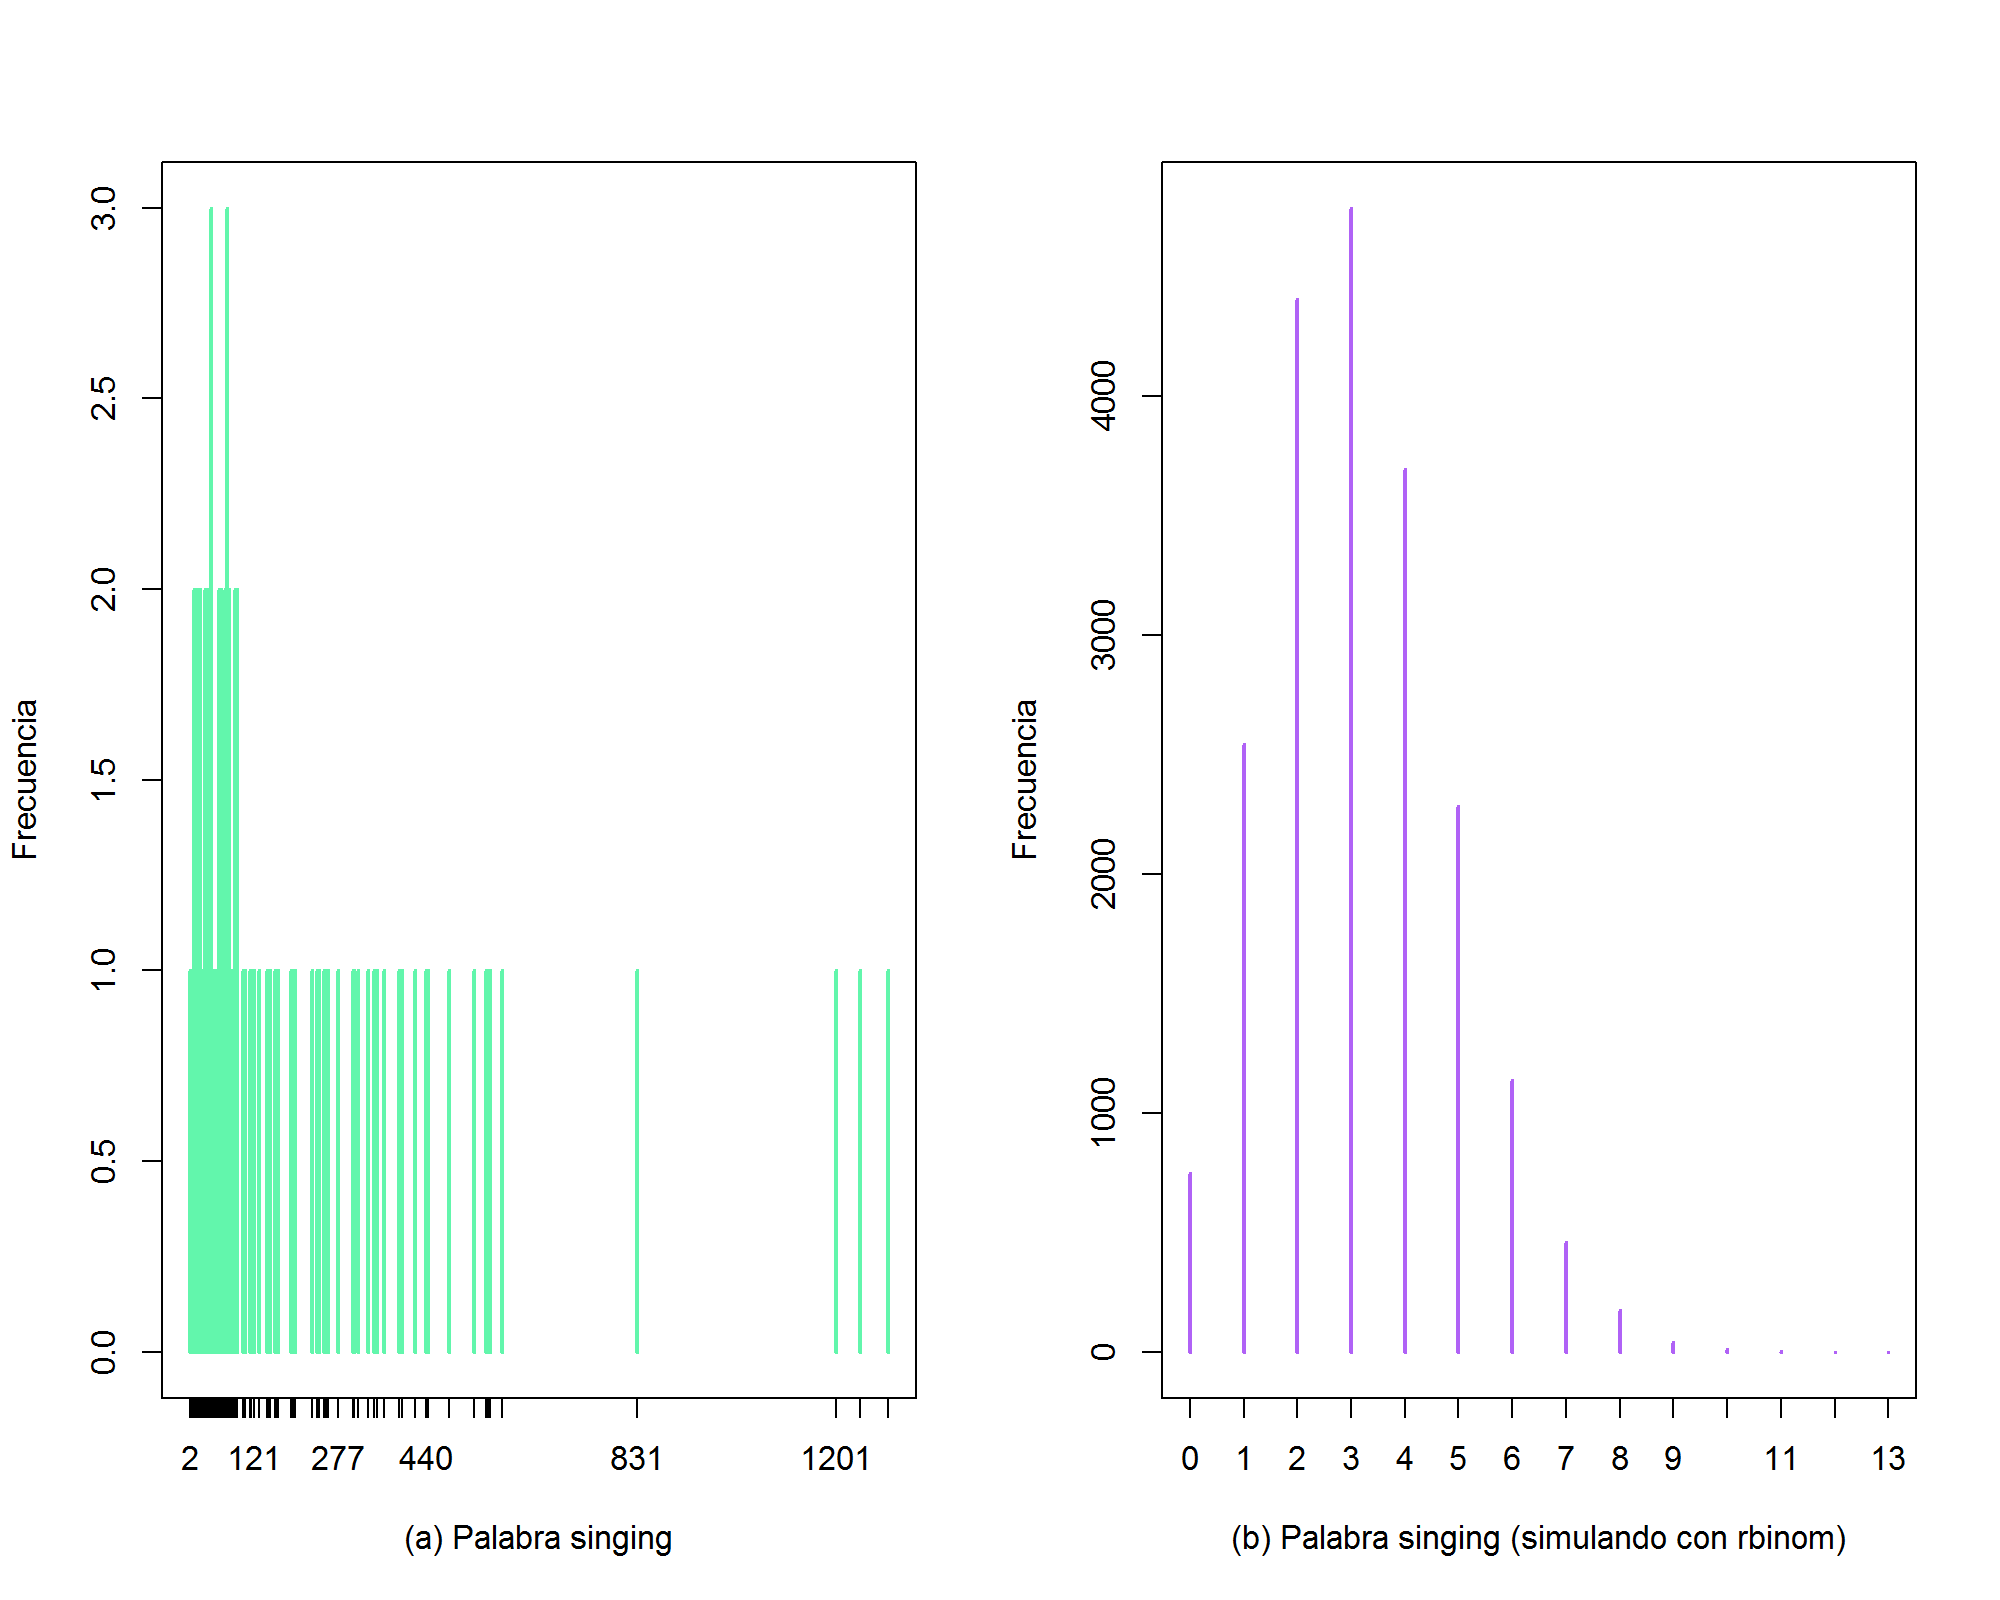
\includegraphics[width=14 cm]{FigModeloReporte/T3_singing_todas.png}
\caption{Frecuencia de la palabra \emph{singing} en el texto}\label{f2}
\end{center}
\end{figure}

En la figura \ref{f3} se puede apreciar la frecuencia con la que fue apareciendo la frase \emph{the singing mouse}, la cual se escogi� por hacer referencia al t�tulo del libro, por lo que se supon�a tendr�a que aparecer bastantes veces en el texto como lo muestra el lado izquierdo de la figura, sin embargo, existen grandes huecos para que vuelva a aparecer, lo que hace suponer que no siga alguna distribuci�n de probabilidad.\\

\begin{figure}[]
\begin{center}
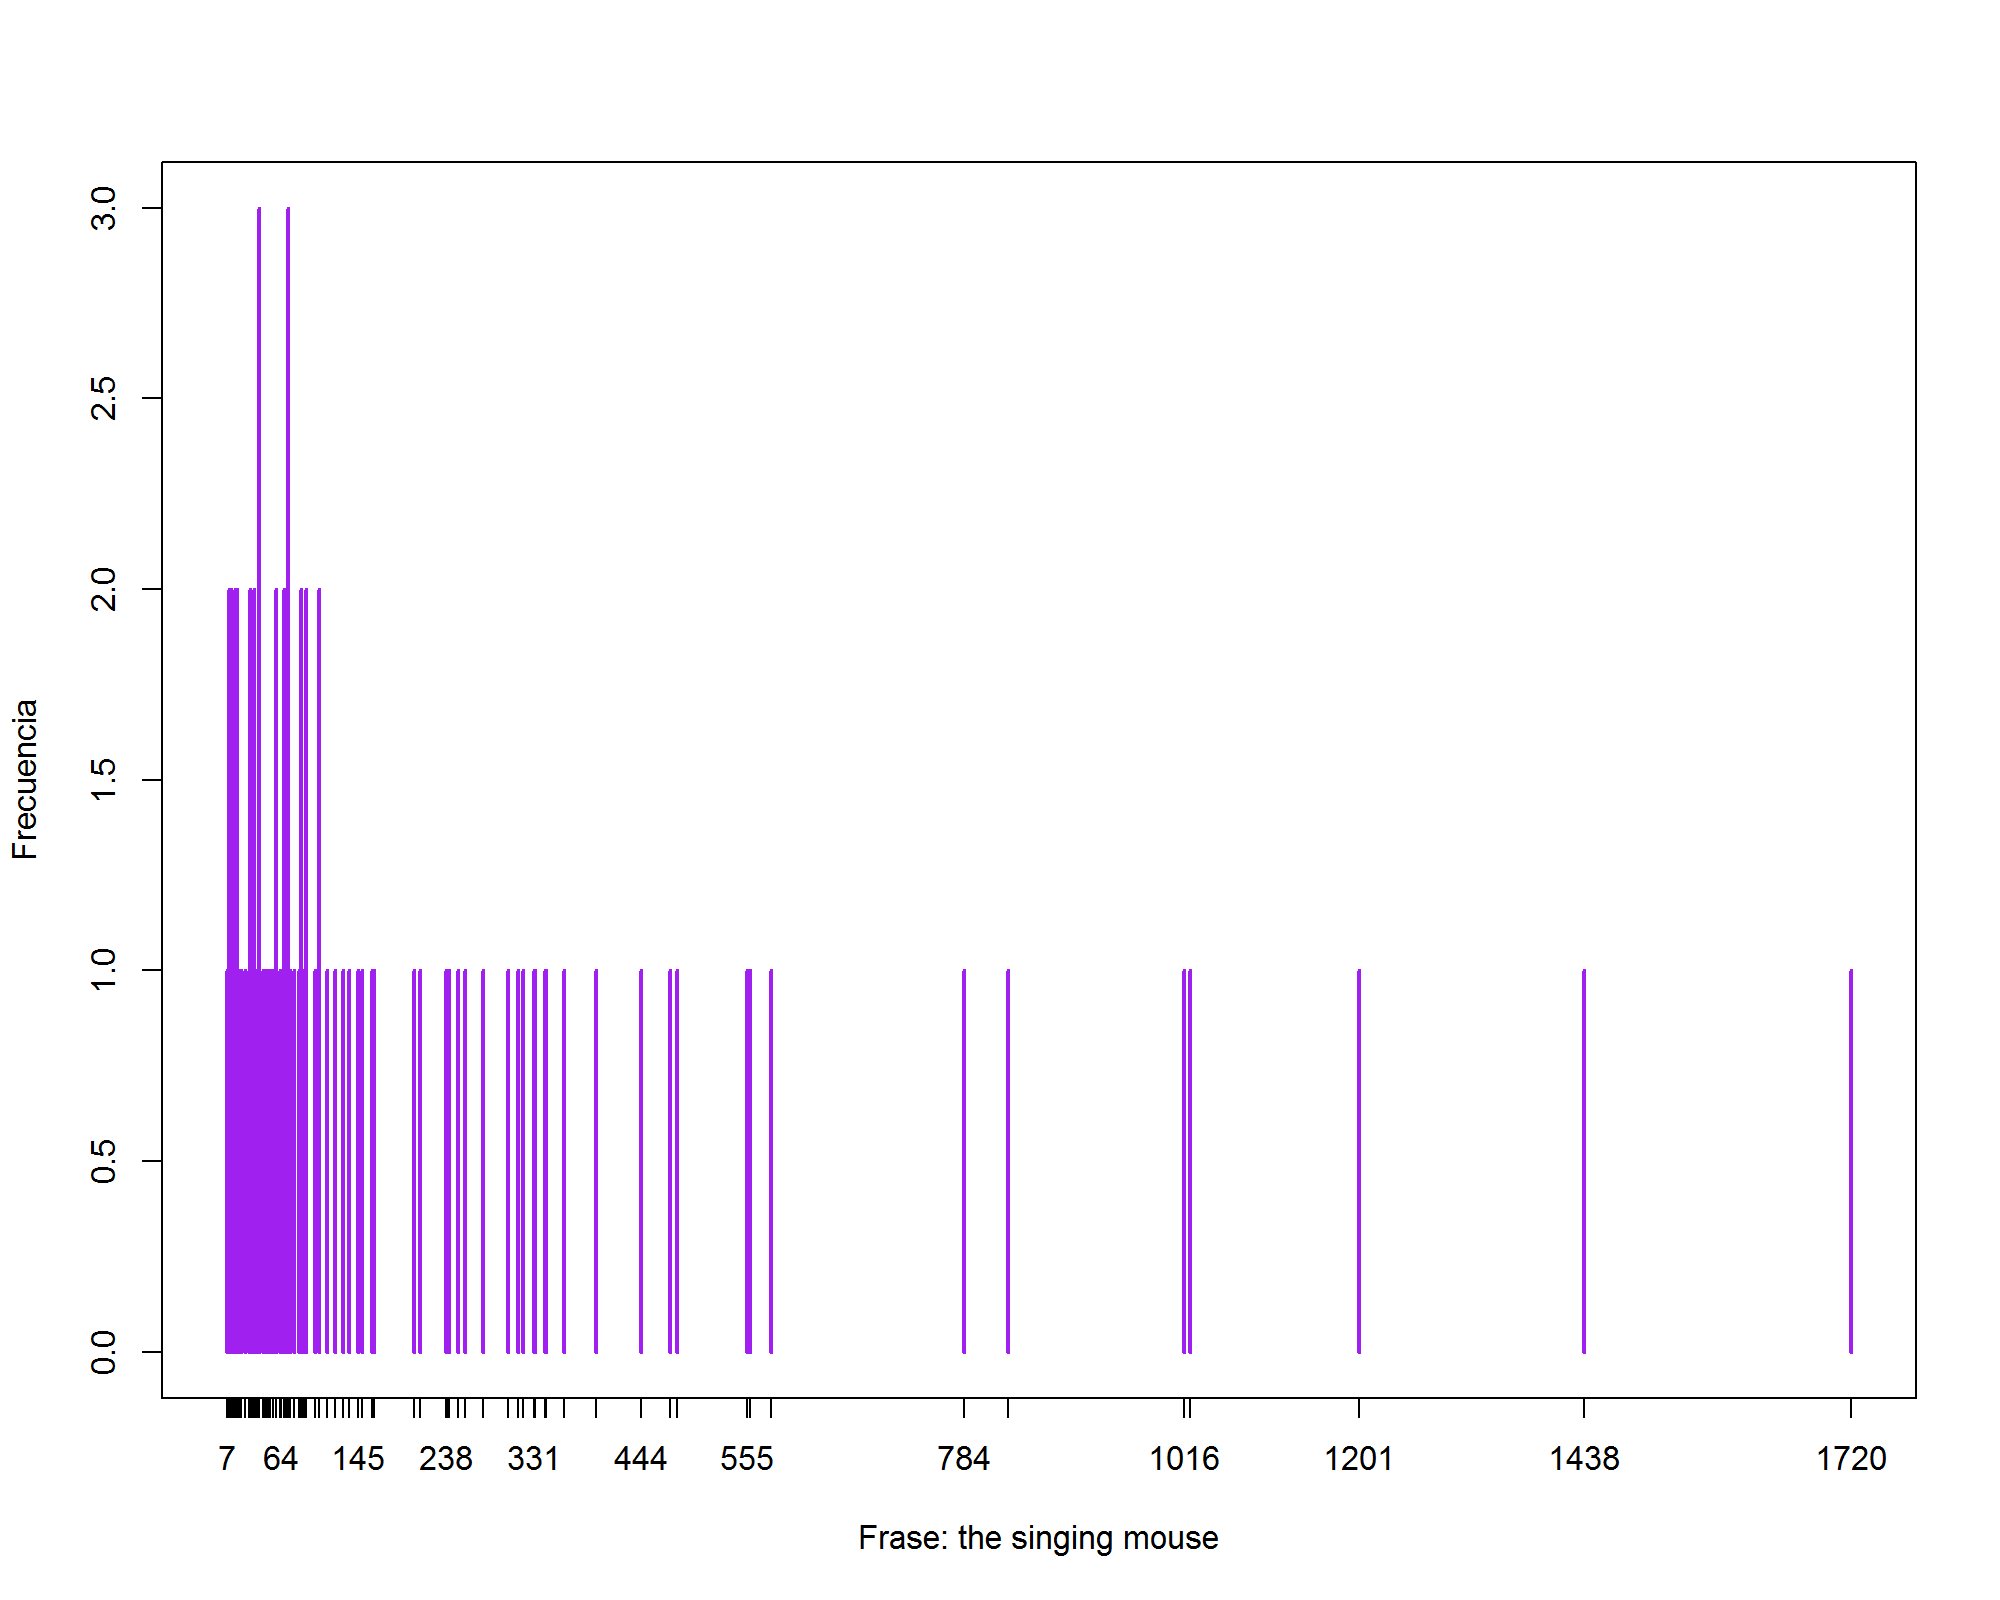
\includegraphics[width=15 cm]{FigModeloReporte/T3_ngram.png}
\caption{Frecuencia de la frase \emph{the singing mouse} en el texto}\label{f3}
\end{center}
\end{figure}

Finalmente, en la figura \ref{f4} se aprecia el comportamiento de la longitud de los trigramas de todo el texto, en donde, se puede apreciar que siguen una distribuci�n Binomial Negativa, ser�a interesante ver el comportamiento de los dem�s ngramas, y ver si se puede concluir con alguna m�trica que pudo haber seguido el autor.

\begin{figure}[]
\begin{center}
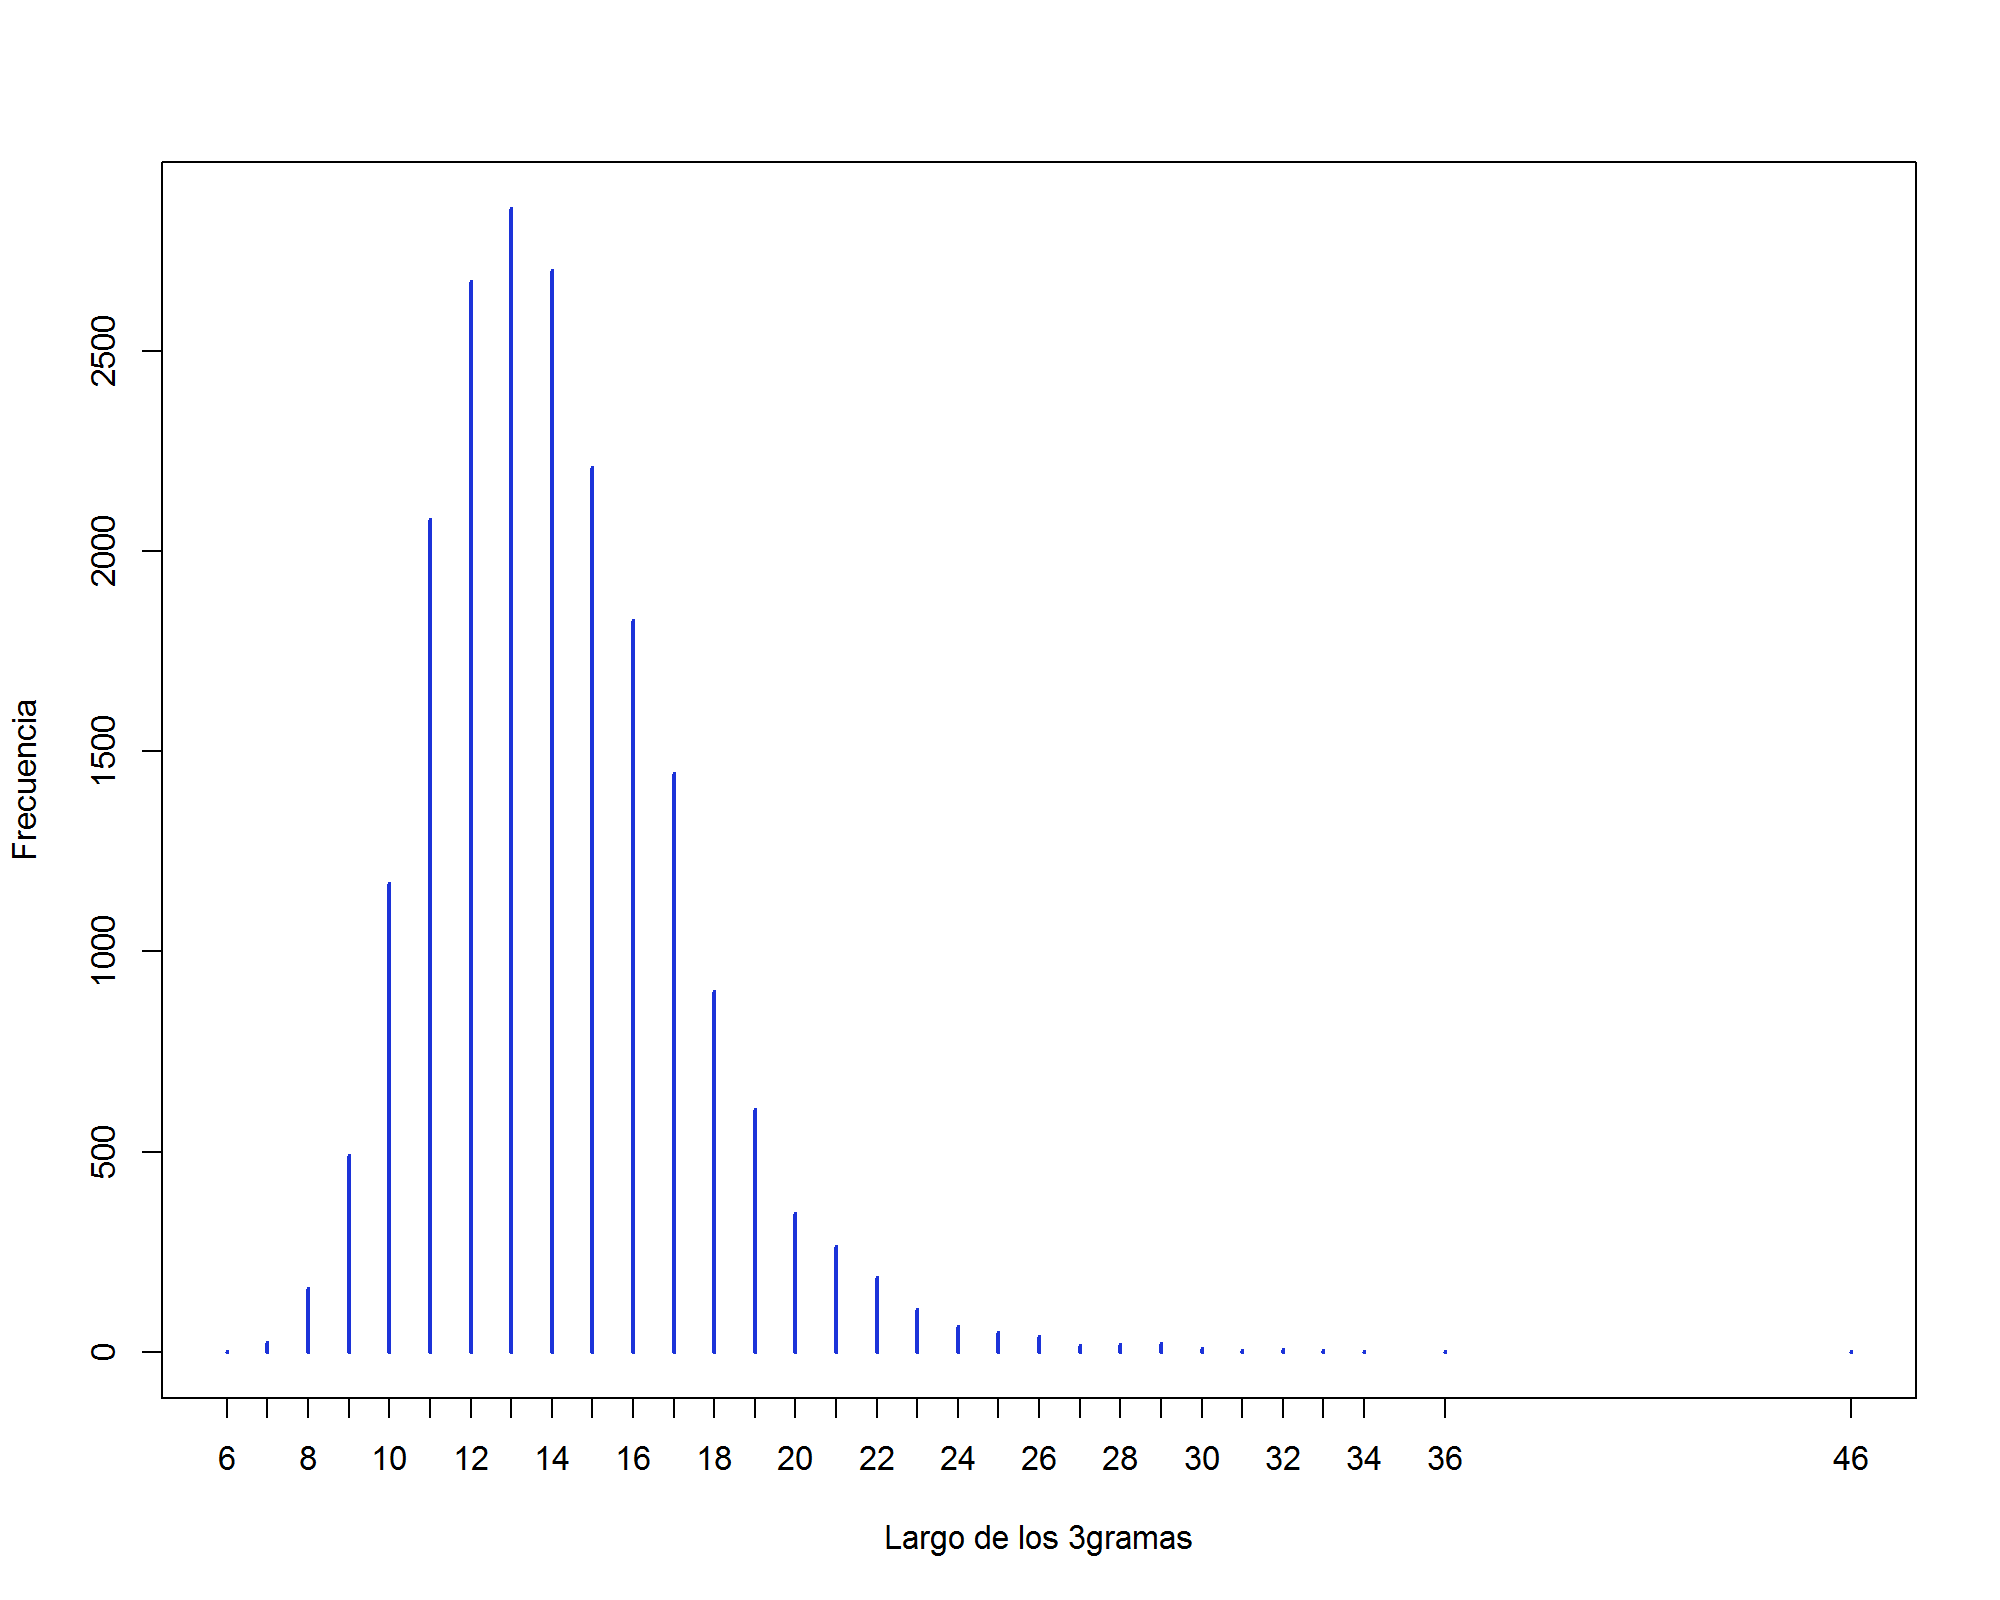
\includegraphics[width=15 cm]{FigModeloReporte/T3_largongram.png}
\caption{Frecuencia del largo de los gramas con $n=3$}\label{f4}
\end{center}
\end{figure}

\bibliographystyle{plain}
\bibliography{MiBiblio}

\end{document} 